\chapter{Deep Learning in Digital Histopathology}

Digitization and technology integration have transformed clinical diagnostics and treatment planning, with histopathology abundantly benefiting from those advancements.
We begin this chapter by introducing the field of histopathology and its concerns, as well as the tools used in contemporary clinical practice.
We illustrate how digitization has helped reduce the logistical complexity of histopathologists' workflow and how decision support systems can further reduce the required amount of human labor.
Finally, we review feedforward artificial neural networks, focusing on convolutional networks, which are particularly suited to various computer vision problems.

\section{Histopathology}

Histopathology is a discipline concerned with the study of diseases of tissues.
The scope of histopathology includes, but is not limited to, the detection and prediction of cancer, the diagnosis of infectious or inflammatory diseases, and the study of brain-degenerative diseases such as Parkinson's or Alzheimer's \cite{histopathology-cancer, histopathology-infectious, histopathology-inflammatory, histopathology-brain-degenerative}.

The Royal College of Pathology \cite{histopathologist-role} defines histopathologists as medically qualified doctors who examine tissue samples from patients.
Their expertise is essential in identifying cellular and tissue anomalies that may indicate various medical conditions.
Histopathologists often work in collaboration with other physicians, providing insights that help guide the direction of further patient care.

\section{Temporal and Spatial Limitations of Traditional Histopathology}

Traditionally, getting tissue from a patient to a histopathologist is a lengthy logistical process involving several people.
The surgeon needs to extract tissue samples from the patient.
As presented in \cite{histo-process}, a specialized laboratory then receives the extracted tissue for processing; technicians infuse the tissue samples with a mix of chemicals and embed them into paraffin wax blocks.
Technicians slice the paraffin blocks into thin sections and laminate those sections onto a glass slide.
They then stain the glass slides with hematoxylin/eosin (or another compound, depending on the use case, as per \cite{histopathology-staining}) to enhance the contrast between different cellular structures.
After the processing, the laboratory sends the slides to a histopathologist for review.

While we cannot replace the surgeons who perform the biopsy or the laboratory workers who stain and embed the tissue, we can address the logistic challenges of moving glass slides to histopathologists.
A physical slide suffers from several inefficiencies. 
Only one or two histopathologists can study a slide at a time.
If a second opinion from a different histopathologist is required, a designated person must transport the glass slide to the respective clinic.
Such logistic pitfalls slow down the diagnostic process and lead to longer waiting times for a patient \cite{from-traditional-to-digital-histopathology}.

\section{Digital Histopathology}

Digital histopathology aims to reduce the logistic overhead caused by physical copies of glass slides.
After the surgeons and technicians extract and prepare the tissue, instead of being sent to a histopathologist, it is scanned using special lenses, resulting in a high-resolution digital image called Whole Slide Image (WSI) \cite{from-traditional-to-digital-histopathology}.
This image is then uploaded to an aggregator server, enabling real-time slide sharing and parallel collaboration of multiple clinicians.
Histopathologists then examine WSI's in a dedicated browser on their computer monitors --- rather than looking at the glass slide under a microscope \cite{digital-histopathology-process}. \myref{Figure}{fig:xopat} shows a WSI of a prostate tissue sample displayed in a dedicated browser developed by the RationAI group.

Although contemporary digital pathology systems significantly speed up pathologist's day-to-day work, we can further optimize another productivity metric: the time a pathologist spends examining WSIs.

\begin{figure}[t]
    \centering
    \fcolorbox{RoyalBlue}{white}{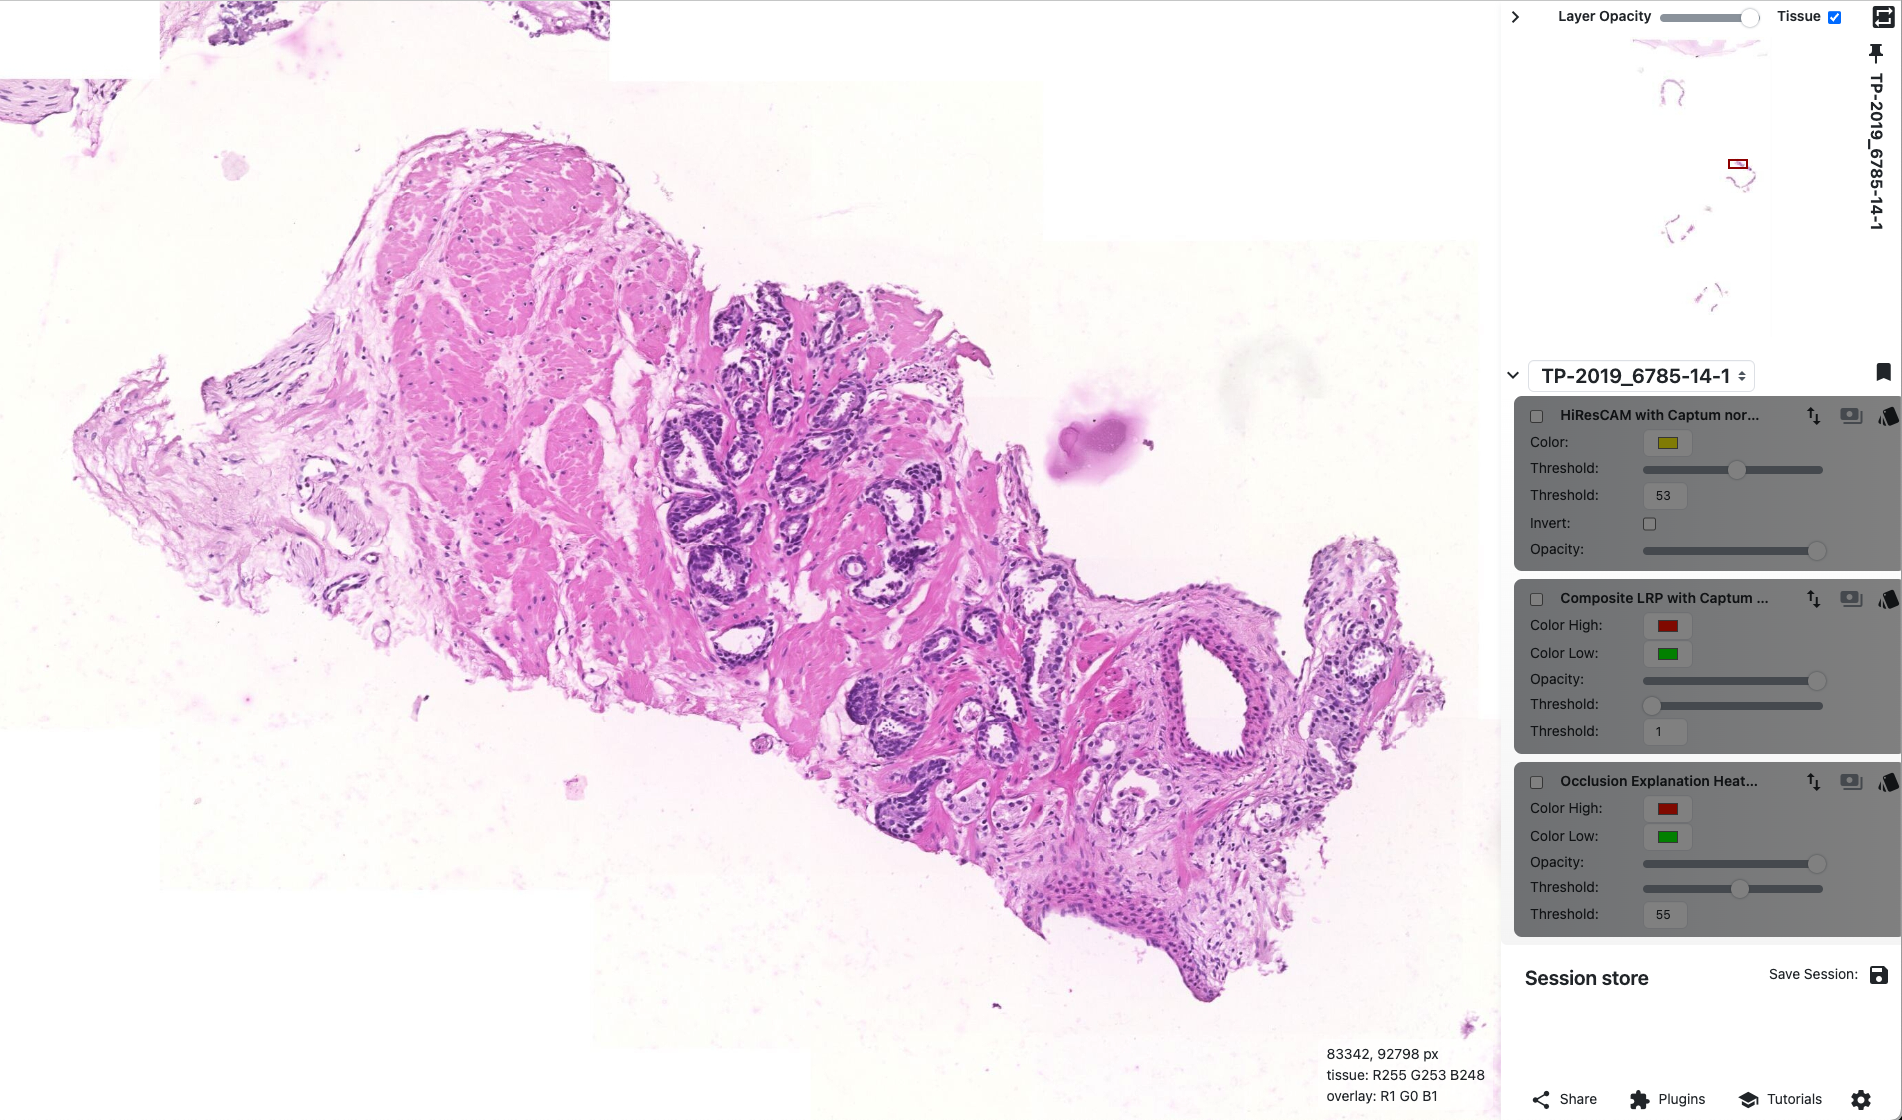
\includegraphics[width=0.97\textwidth]{img/xopat.png}}
    \caption{xOpat \cite{xopat} WSI browser with a sample of prostate tissue. The histopathologist can move and zoom the tissue, allowing him to navigate the WSI quickly. Digitized copies allow for the layering of arbitrary annotations on top of the WSI, providing great collaborative capabilities. For example, different pathologists can mark cancerous regions and then display them on top of each other to see their agreement.}
    \label{fig:xopat}
\end{figure}

\subsection*{Decision Support System}

A decision support system is a computer system that assists humans in making decisions while performing a particular task.
These systems are used in various domains, including high-stake environments such as investment banking, autonomous driving, or military and defense \cite{dss-finance, dss-autonomous-driving, dss-military-and-defense}.
In digital histopathology, clinicians typically use such systems to support operational processes \cite{digital-histopathology-process}.
However, with deep learning in the spotlight of today's research, new possibilities are emerging.

Systems based on deep learning could improve the tissue diagnostic process by assisting diagnosis or discovering previously unrecognized features in large sets of data that are beyond the comprehension of a single expert \cite{dss-digital-histopathology}. 
Researchers and various companies are actively trying to use machine learning systems in this way. 
These systems often provide results in real-time and domain-expert-like performance, demonstrating that further research can significantly improve current processes \cite{deep-learning-in-histopathology}.

\section{Deep Learning}\label{section:dl}

The branch of machine learning that encapsulates neural networks (NNs) is called deep learning (DL).
The methods and algorithms used by DL achieve remarkable results in various fields such as computer vision, games, or weather forecast \cite{alexnet, alphago, weather}. The following parts provide an overview of the necessary concepts used in this work and are drawn from the work of Goodfellow et al. \cite{goodfellow}.

\subsection*{Feedforward Neural Network}\label{feedforward-nn}

Feedforward networks are considered the starting point of modern DL models.
They get their name from the unidirectional flow of information within the network.
We can think of feedforward networks as a function $f$ that maps input vector $x$ from input space to a value $y$ from output space.
Throughout this thesis, we will only consider this type of network.

A common approach to studying neural network architectures is to see them as a sequence of layers.
Each layer $l$ resembles an intermediate function $f^l$.
Let our network be a composition of $L$ layers numbered from $1$ to $L$.
For any given input vector $x$, the computation performed by the network can be expressed as a composition of its intermediate layer functions, yielding
\begin{equation}
    f(x) = f^L(f^{L-1}(\cdots f^1(x))).
\end{equation}
In this notation, layer $1$ is the input layer, which receives the input vector $x$.
The last or $L$-th layer is the output layer, which returns the network's prediction or decision $y$.
All intermediate layers are called hidden layers and transform one internal representation into another.

Although \cite{cybenko} essentially shows that one hidden layer is all you need, neural networks typically employ multiple hidden layers.
The motivation is that we think of each layer as capturing certain abstractions or representations from its input.
Deeper layers can, therefore, build more complex representations using abstractions captured by previous layers.

Multi-layer Perceptron (MLP) is a fundamental architecture in the history of feedforward neural networks.
In an MLP, the basic building block is a neuron.
Neurons are arranged in layers to form the final network.
A neuron receives input signals (input features $x$), processes them, and outputs its signal ($y$), which is passed on to subsequent neurons in the following layer.
The processing consists of calculating the inner potential $\xi$, a weighted sum of the neuron's inputs.
The inner potential is then passed to the activation function, denoted as $\sigma$. 
Given a neuron $i$ expecting $K$ input signals, with activation function $\sigma_i$, the output signal $y_i$ is expressed as
\begin{equation}
    y_i = \sigma_i(b_i + \sum_{k=1}^K w_{ik}x_k)
\end{equation}
where weight $w_{ik}$ connects $k$-th input feature to the neuron $i$ and $b_i$ is a constant bias term, improving the neuron's modeling capabilities.
If all neurons in a given layer $l$ have incoming weights from all neurons in the previous layer, we say that $l$ is fully connected (FC).
% \myref{Figure}{fig:simple-mlp} depicts a small MLP with one hidden layer.

Weights and biases are called trainable parameters. %, denoted as $\theta$.
Deep learning aims to make the trainable parameters useful.
A a network computes a function $f$, with specific training, we can make the network configure its parameters to approximate a desired function $f^*$ within a certain tolerance.
To configure the parameters, we leverage a large amount of data to minimize the difference between $f$ and $f^*$.
The difference is captured by a loss function $\ell$, and minimizing $\ell$ is typically performed iteratively using backpropagation and training algorithms such as stochastic gradient descent.
More on neural network training can be found in \cite{goodfellow}.

Even though MLPs demonstrate impressive results on tasks previously deemed impossible for computers, they have certain drawbacks.
If we used only FC layers, contemporary architectures such as AlexNet from \cite{alexnet} would have an unimaginable number of trainable parameters.
This led to the development of new architectures tailored to specific domain needs.

\subsection*{Convolutional Neural Network}
Convolutional Neural Networks (CNNs) focus on working with grid-like data.
Therefore, their input $x$ typically comes in the form of a multidimensional array of shape $H \times W \times C$, where $H$ and $W$ stand for height and width respectively, and $C$ is the number of channels ($1$ for grayscale images, $3$ for RGB images).
CNNs have been introduced specifically to solve various computer vision problems and add two additional layer types --- convolutional and pooling.
These layers help capture patterns in the input features and reduce the size of the network \cite{cnns}. 

\subsubsection{Convolutional Layer}

The convolutional layer uses trainable filters (kernels) to search for visual patterns in its features.
The filter is typically smaller in width and height than the input but spans all the input channels.
Rather than interacting with the entire input at once using weighted connections, the filter $F$ is systematically slid across the input, and the filter weights convolve with the corresponding input data segments, resulting in a two-dimensional \emph{activation map} $A$.
Convolution is a linear operation that chains the element-wise product of the filter and its receptive field over all channels and then sums the products into one value. Given a filter $F$ and input $I$, the spatial activation $A_{ij}$ is computed as 
\begin{equation}
    (F * I)_{ij} = b + \sum_{x=0}^{H-1} \sum_{y=0}^{W-1} \sum_{z=0}^{C-1} F_{xyz} \cdot I_{(i+x)(j+y)z}
\end{equation}
where $W$, $H$ are width and height of $F$ and $C$ is number of input channels. The bias term $b$ is used similarly as in the case of fully connected layers.

The resulting activation map can be thought of as a map of evidence for the presence of a shape detected by the filter in the input data.
Sliding the filter through features gives us spatial invariance --- no matter where the learned pattern resides in the input, it will be detected and reflected in the corresponding activation map, something very hard to achieve using a fully connected layer.
Therefore, we commonly say the filter has \emph{shared weights}, as per \cite{goodfellow}.
Sharing weights has not only effects of identifying patterns regardless of their position in the input --- it also reduces the number of parameters we have in the network.

When incorporating a convolutional layer into a neural network, the critical parameter to define is the shape of the filter.
The shape determines the size of the receptive field -- how many input features the filter can see at a given position.
In addition, we usually set two other parameters: \emph{padding} and \emph{stride}.
Padding is a value we add as a border around the input features, allowing the filter to cover the edges and thus reduce information loss.
Stride controls how much we move the filter after each convolution.

A convolutional layer typically consists of several units.
Each unit has its filter and produces a unique activation map.
The idea is that each filter learns to recognize a different pattern during training --- and each unit produces a map of evidence of its detected pattern.
This gives a single layer the capability to detect multiple patterns, and, similarly to its fully connected counterpart, it allows subsequent layers of the network to build upon captured abstractions and ultimately ``understand'' and represent high-level concepts.
Given a convolutional layer, we will denote its $k$-th activation map as $A^k$.


\subsubsection{Pooling Layer}

To avoid overfitting the network, we employ pooling layers to distill captured patterns.
They progressively reduce the size of the input features, leading to a smaller number of model parameters and reduced computational time, per \cite{cnns}.

A pooling layer is typically placed after a convolutional one, iterating its activation maps and systematically applying a specific operation over its receptive field.
We differentiate between two primary types of pooling: \emph{max} and \emph{average}.
As their names suggest, max pooling selects the maximum value within its receptive field, while average pooling calculates the average of the values.

\subsubsection{Global Pooling Layer}

Given that our network comprises only convolutional and pooling layers, we are not bound to any specific input size.
However, as noted in \cite{cnns}, it is common practice to introduce fully connected layers towards the end of a network, which requires a fixed number of input features.
To meet this requirement, we use global pooling layers.

The global pooling layer condenses each activation map into a single value.
This guarantees that if a convolutional layer has $n$ units and the subsequent fully connected layer receives $n$ input features, placing a global pooling layer in between will provide a compatible transition, standardizing the output size of the last convolutional or pooling layer regardless of the original input data dimensions.

Throughout this thesis, we will denote globally pooled activation map $A^k$ as $a^k$. For a global average pooling (GAP) layer, the $a^k$ is computed as
\begin{equation}\label{gap}
    a^k = \frac{1}{|A^k|} \sum_{i=0}^{H-1} \sum_{j=0}^{W-1} A^k_{ij}
\end{equation}
where $|A^k|$ represents the number of spatial activations in the activation map $A^k$.
For the global max pooling (GMP), the \myref{Equation}{gap} changes to
\begin{equation}
    a^k = \max_{i,j} A^k_{ij}.
\end{equation}